\chapter{A Review of Methods To-Date}

The GALAH survey is not biased towards emission-line stars and it is expected that a majority of spectra are typical. This posses a challenge and constraint on the methods that can be used to identify emission-line spectra. As such methods must be adapted to detect anomalies or outliers in data in order to separate emission-line spectra from more typical spectra. In this work, identifying emission-line spectra in large scale surveys is presented as a pre-processing step to classification. It forms a critical step in the novel method presented in Chapter 6. 

This chapter presents essential background material and a review of methods and methods that have been used to identify H$\upalpha$ emission-line spectra, in both smaller scale observations during the latter half of the 20th century as well as more modern large scale surveys in the early 21st century. These methods have also been placed in the context of their importance in the identification and classification of P Cygni, inverse P Cygni and other emission-line spectra.

\section{A Historical Perspective}
In Chapter 1, this work introduced the work of Beals who pioneered the study of emission-line stars in the 20th century. The work was manual, time consuming and took the researcher decades to compile\cite{1953PDAO....9....1B} with the assistance of a team that included secretaries and draftspersons. Despite these efforts, the catalogue of data compiled in 1953 was small by modern standards. This work could not identify more work in literature that focused on identifying and classifying emission-line stars until the late period of the 20th century. This is potentially due to the significant amounts of labour required to carry out these proects with the absence of modern data mining methods. 

In terms of this work, an atlas of high resolution line profiles with H$\upalpha$ emission-line spectra was provided by Van Winckel at al. in 1993\cite{van1993atlas}. The authors note that the radial velocities of the 59 emission lines considered were generally red-shifted. They provide a classification scheme for H$\upalpha$ spectra based on their morphology, devised entirely by using manual methods. More specifically, direct visual inspection and measurement of the width and shape of the line profile was used to classify these spectra. In particular, wind velocity dispersion outside the primary disk of the star was used to determine the membership of spectra in each class.

\begin{figure}[!htb]
\centering
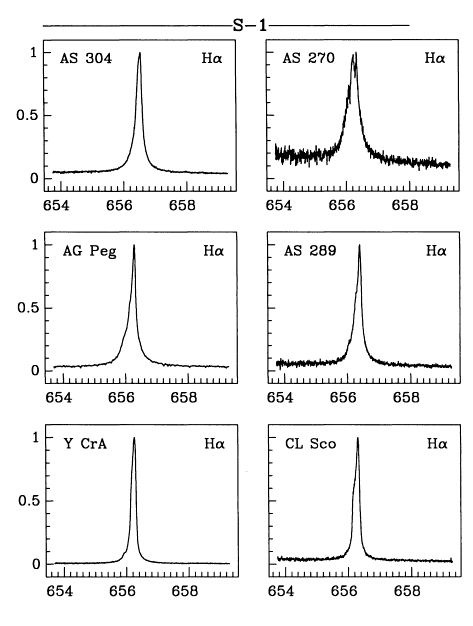
\includegraphics[scale=0.75]{figures/van winckel class.png}
\caption{Sample spectra from sub-type S1 as classified by Van Winckel et al. (reproduced).}
\end{figure}

\begin{figure}[!htb]
\centering
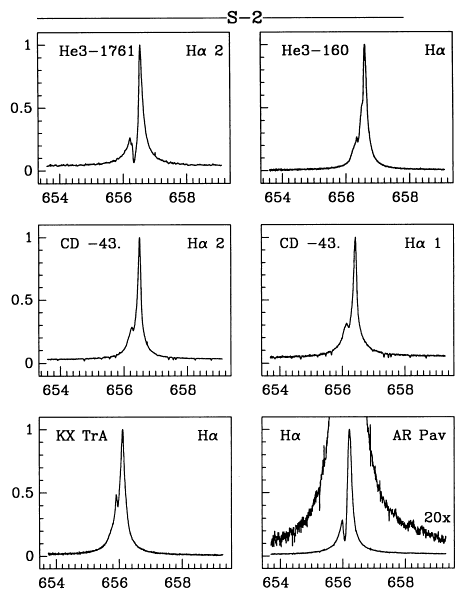
\includegraphics[scale=0.75]{figures/van.png}
\caption{Sample spectra from sub-type S2 as classified by Van Winckel et al. (reproduced).}
\end{figure}

A few of the classes identified by the authors include, sub-type S1, which are narrow emissions with no prominent absorption; sub-type S2 which shows a clear absorption feature superimposed on a broad emission feature; and sub-type S3 which shows a strong absorption feature which reaches at least the continuum level. S3 showed the smallest wind velocity dispersion, thus demonstrating the relationship between the morphology of the spectra and the physical processes that generate them.

\begin{figure}[!htb]
\centering
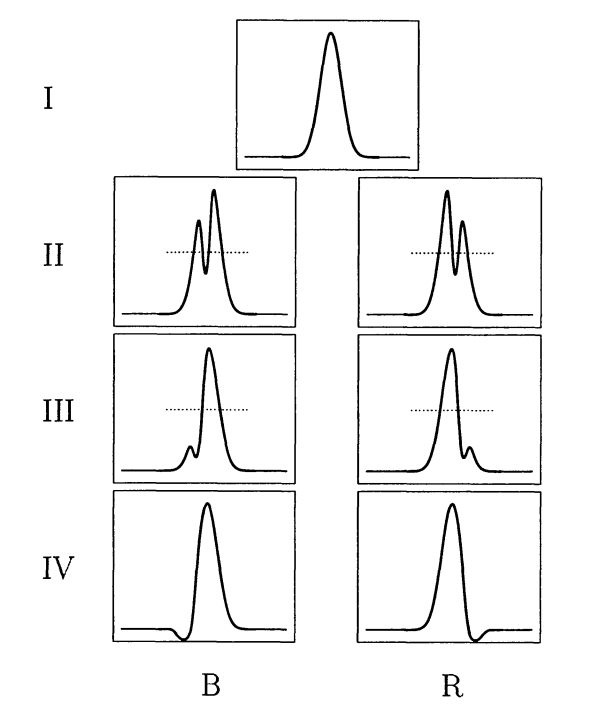
\includegraphics[scale=1]{figures/reipurth classes.png}
\caption{The morphology based classification scheme proposed by Reipurth et al. (reproduced). Depending on the location of the primary peak in relation to the secondary peak, the letters B and R were appended to the Roman numerals. They stand for blue-shifted and red-shifted respectively.}
\end{figure}

Following on three years later, in 1996, Reipurth et al. studied the H$\upalpha$ emission-line profiles of pre-main sequence stars using manual methods. In addition to identifying T Tauri stars and Ae\symbol{92}Be stars using high resolution spectra (R$\sim$50,000), the study focused on the morphological properties of P Cygni stars as well as the physical processes that generate them. The study notes the discovery of complex morphological profiles among the T Tauri, Ae\symbol{92}Be and P Cygni stars. 

The authors proposed a two dimensional classification scheme based on the relative height of a secondary peak compared to the primary peak, and whether the absorption line is blue or red shifted. The authors note the classification of 25\% symmetric profiles, 49\% blue shifted absorption profiles and 5\% P-Cygni profiles amongst the observed spectra. Of the spectra, 21\% fall into the red-shifted absorption category. In addition to this morphological classification, the authors also presented wind velocities of the samples with some stars recording extremely high velocities of $\sim$900km/s\cite{reipurth1996halpha}. 

The classification of P Cygni stars in Reipurth et al. follows the scheme proposed by Beals in 1953\cite{1953PDAO....9....1B}. The authors have also presented a discussion comparing observed data to models in literature, particularly models that constrain mass, radii and photospheric temperatures. No specific model details for P Cygni stars were provided. Further catalogues of H$\upalpha$ emission-line stars have been provided by Kohoutek and Wehmeyer (1997 and 1999). These catalogues contain 98 identified emission-line stars in the Northern Milky Way. These catalogues do not specifically identify P Cygni stars or inverse P Cygni stars\cite{kohoutek1999catalogue}.

Working with data from NGC 6611, in 2013, Bonito et al.\cite{bonito2013spectroscopic} note that for stars surrounded by active disks, the morphology of the emission lines could fall into categories such as symmetric with broad wings, asymmetric and in extreme cases, P Cygni and inverse P Cygni. The authors have used the classification scheme proposed by Reipurth et al. mentioned above and have adhered to the type I - IV scheme with B and R suffixes to denote blue-shifted and red-shifted emission lines respectively. 
Traven et al. presented a catalogueue of H$\upalpha$ emission-line stars in the Gaia-ESO survey. This survey is biased towards young open clusters and consequently, the authors note a relatively large proportion of H$\upalpha$ emission-line spectra that were identified in this work. The authors note the identification of 3765 emission-line stars from a sample of 22,035 spectra from the Gaia-ESO survey. This work is notable as it uses a combination of empirical rules and automated methods like spectral fitting to sort the H$\upalpha$ emission-line spectra into eight distinct morphological categories: single–component emission, emission blend, sharp emission peaks, double emission, P-Cygni, inverted P-Cygni, self–absorption, and emission in absorption\cite{traven2015gaia}. These were briefly presented in Chapter 1.

\begin{figure}[!htb]
\centering
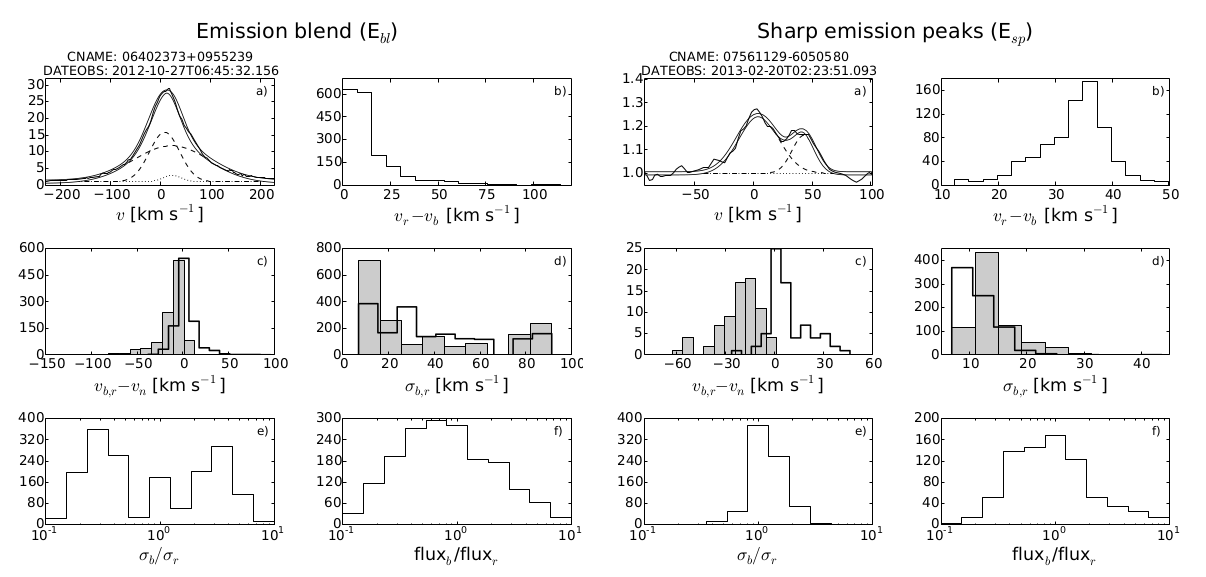
\includegraphics[scale=.50]{figures/gaia eso1.png}
\caption{Classes of emission-line spectra identified in the Gaia-ESO Survey. Reproduced from Traven et al.}
\end{figure}

\begin{figure}[!htb]
\centering
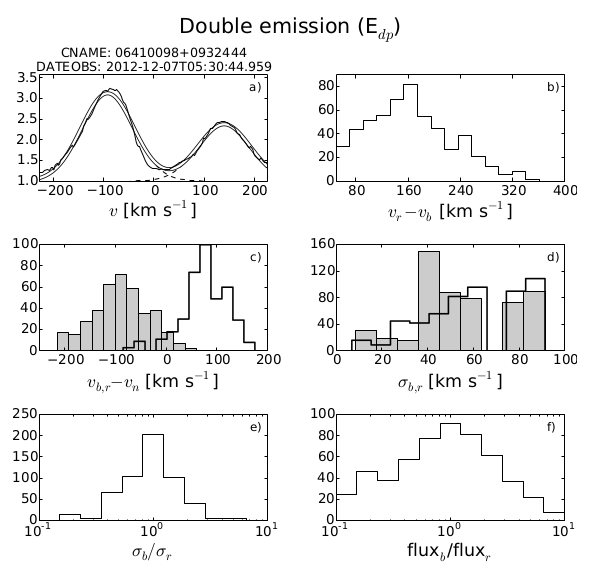
\includegraphics[scale=.50]{figures/gaia eso2.png}
\caption{Classes of emission-line spectra identified in the Gaia-ESO Survey. Reproduced from Traven et al.}
\end{figure}

The Gaia-ESO survey had conducted repeat observations of about half the identified H$\upalpha$ emission-line stars. Thus the authors were able to comment on the temporal variability of these stars. The conclusion was that while some morphological categories exhibited stability of their spectral profiles over time, P-Cygni and self-absorption profiles may not. Supplementary information of these spectra from SIMBAD, VizieR and ADS were also provided. In addition to this data, the authors have provided wind velocity estimates based on the curve fitting procedure. The authors note that the identification, classification and characterisation of emission-line stars can be valuable for automatic pipelines in large surveys, where they can pinpoint outliers when calculating general stellar properties and abundances. Additionally, they note that the identified stars can be used in studies of star formation processes, interacting binaries and related fields of stellar physics. 

This work draws several conclusions from this historical perspective,

\begin{enumerate}
\item These methods relied exclusively on visual inspection of spectra and manual methods to identify H$\upalpha$ emission-line spectra. While this may have been a suitable approach in the past, it is extremely challenging to extend and scale these methods to data sets generated by million star all sky surveys in the modern era.

\item It was demonstrated in Chapter 1 that the variety of spectral morphologies are hypothesised to be generated by distinct physical phenomena linked to the stellar disk and the gas that surrounds it. Thus morphology based classification approaches as demonstrated by Reipurth et al. and Beals are imporant in the context of developing a greater understanding of stellar evolution and dynamics.

\item Finally, these studies have identified P Cygni and inverse P Cygni (among other classes of spectra) as a subset of H$\upalpha$ emission-line spectra. The current work takes this fact to its logical conclusion i.e. the probability identification of P Cygni and inverse P Cygni spectra can be increased if the search space and feature space of the raw data can be reduced from the complete DR3 catalogue, to a much narrower subset of H$\upalpha$ emission-line spectra during pre-processing. 
\end{enumerate}

\section{Recent Developments}

The increase in data availability via large scale spectroscopic surveys has necessitated and demanded the use of semi automated and fully automated detection and identification methods. More recently, these methods have included statistical analysis and machine learning. In general, machine learning approaches can fall into two categories; supervised and unsupervised learning. The former relies on the availability of a suitably robust set of training examples while the latter attempts to generalise and learn from unlabelled data\cite{hastie2009elements}. 

While a full discussion and review of machine learning methods is beyond the scope of this thesis, the methods that are relevant to this work are presented in text in subsequent chapters, with Chapter 4 in particular presenting a more detailed discussion on methods that are relevant to this work. This section following reviews four recent methods that use machine learning to identify spectra in large surveys and discusses their strengths and limitations.

\subsection{Applying K-means Clustering Directly on Data from the APOGEE Survey}

K-means clustering is a well known unsupervised clustering algorithm. The goal of this algorithm is to partition a set of observations into a predefined set of clusters. Each observation would belong to a cluster with the nearest mean which serves as the centroid or prototype of the cluster\cite{macqueen1967some}. Formally, given a set of $n$ observations such as \(x_1,x_2,...,x_n\) where each observation is a $d$ dimensional vector, the algorithm will partition the $n$ observations into $k$ sets $S=\{S_1,S_2,...,S_k\}$ such that the intra-cluster variance is minimised. This objective can be represented as,

\begin{equation}
{\underset {\mathbf {S} }{\operatorname {arg\,min} }}\sum _{i=1}^{k}\sum _{\mathbf {x} \in S_{i}}\left\|\mathbf {x} -{\boldsymbol {\mu }}_{i}\right\|^{2}={\underset {\mathbf {S} }{\operatorname {arg\,min} }}\sum _{i=1}^{k}|S_{i}|\operatorname {Var} S_{i}
\end{equation}

where $\mu_i$ is the mean of the points in $S_i$. 

Using the identity,

\begin{equation}
    |S_{i}|\sum _{\mathbf {x} \in S_{i}}\left\|\mathbf {x} -{\boldsymbol {\mu }}_{i}\right\|^{2}=\sum _{\mathbf {x} \neq \mathbf {y} \in S_{i}}\left\|\mathbf {x} -\mathbf {y} \right\|^{2}
\end{equation}

It can be shown that this is equivalent to minimising the pairwise squared deviations of points belonging to the same cluster,

\begin{equation}
{\underset {\mathbf {S} }{\operatorname {arg\,min} }}\sum _{i=1}^{k}\,{\frac {1}{|S_{i}|}}\,\sum _{\mathbf {x} ,\mathbf {y} \in S_{i}}\left\|\mathbf {x} -\mathbf {y} \right\|^{2}
\end{equation}

This method was used on high resolution APOGEE data (R$\sim$22,500), which is part of the Sloan Digital Sky Survey (SDSS)\cite{eisenstein2001spectroscopic}\cite{blanton2017sloan}. In the absence of labelled training samples in the APOGEE survey, Garcia-Dias et al. used k-means to cluster similar spectra into distinct groups\cite{garcia2018machine}. Each spectrum produced by APOGEE was treated as a $d$-dimensional vector. The number of observations $n$ was the number of spectra generated by APOGEE which was approximately 150,000. $k$ was set to 50, presumably by a process of trial and error. The authors note that they were able to separate dwarfs, sub-giants, RC and RGB stars using this approach. The authors note that the approach is sensitive to initialisation and thus sensitive to the number of clusters $k$. One major limitation of this approach is that a discrete classification in the flux space does not result in a neat organisation in the parameters' space, which implies that the authors' were not able to link spectral features such as morphologies to the machine learning parameter space. The other imitation is the manual sorting of clusters that reduced the number of clusters from 50 to 9. This implies that certain spectra were incorrectly clustered by the k-means algorithm. Notable, the authors were unable to cluster H$\upalpha$ emission-line spectra using this method. 

The primary conclusion that can be drawn from this work is that k-means clustering, while robust on more traditional machine learning tasks, may perform poorly if it is used to cluster and ultimately classify morphologically similar spectra such as P Cygni, inverse P Cygni and other emission-line classes identified using manual methods. A method that relates the flux space, and consequently the morphology of the spectrum, to a parameter space may perform better than k-means. 

\subsection{Combining Machine Learning and Manual Methods on Data from the LAMOST Survey}

The LAMOST survey is a low resolution spectroscopic survey with 10 million Milky Way stars as potential survey spectra. Zhang et al. were able to use a training and test set (labelled spectra) comprising of 5915 samples for spectral classification. This training set was based on data released by Hou et al.\cite{hou2016catalog}, who developed the data set by using a combination of empirical rules and visual examination of 10,000 LAMOST spectra. The existence of labelled data including seven P Cygni and inverse P Cygni spectra identified by Hou et al. was used by Zhang et al. for supervised machine learning algorithms.Ten different supervised learning methods were then applied to this data set including including KNN (K-Nearest Neighbor), RF (Random Forest), AdaBoost, Naive Bayes (MultinomialNB, GaussianNB, BernoulliNB), logistic regression, SVM (Support Vector Machine) and Artificial Neural Network (Single-hidden Layer, Three-hidden Layer)\cite{zhang2021catalog}. A comparison of the performance of these methods was not provided by the authors. A detailed discussion of these methods is omitted as it would be beyond the scope of this thesis. 

Zhang et al. note that the k-nearest neighbour and random forest methods outperformed all other methods. These two supervised machine learning models were then applied to 498,588 spectra resulting in 56,574 potential H$\upalpha$ emission-line spectra. These spectra were then visually inspected with a final candidate list of 30,048 H$\upalpha$ emission-line spectra. Despite the use of a number of machine learning methods, the authors fell back on manual visual inspection of spectra in building the training set as well as during classification of the identified potential H$\upalpha$ emission-line spectra.

\subsection{Dimensionality Reduction In Action: Using t-SNE to Classify GALAH DR1 Spectra}

As discussed previously, a stellar spectrum of vector length $d$ (a wavelength grid of size $d$), can be used to create a vector space of dimensionality equal to $d$. In the case of GALAH DR1 this value is $\sim$4500.Conducting computational operations such as clustering and classification on a higher dimensional vector space of size $\sim$4500 can be challenging as it introduces significant computational overheads. In addition to the previously mentioned curse of dimensionality, researchers would also face practical limitations due to the computational intractability of working on higher dimensional vector spaces.

It is often helpful to transform the data from a high-dimensional space to a low-dimensional space while ensuring that meaningful features of the original data are preserved. In the case of P Cygni and inverse P Cygni spectra, these meaningful properties would presumably include some information about the morphology of the spectrum although this may not be guaranteed. This work will revisit this in detail in Chapter 5.

Given a total feature space (and consequently a total search space) that is made up of $n$ spectra samples of length $d$, dimensionality reduction offers an attractive approach to grapple with the curse of dimensionality and high computational complexity. Principal component analysis (PCA) is arguably the most well known dimensionality reduction method. However, PCA may not be suitable in the context of GALAH DR1 and certainly DR3 since these data sets are biased towards non-emission line spectra. Thus a PCA led approach may select features that represent the absorption-line, while emission-line features may not be considered a principal component. This hints at a possible outlier or anomaly detection based approach to emission-line spectra identification. This work will revisit this idea in Chapter 6.

More recent and novel dimensionality reduction methods such as t-distributed stochastic neighbour embedding (t-SNE)\cite{van2008visualizing} have been used on spectral data from GALAH DR1\cite{traven2017galah}. Given a vector of size $d$, the application of the t-SNE algorithm will project this vector space onto a 2-dimensional vector space. The distances between data points on this 2-dimensional vector space can then be used to cluster similar data points into similar groups using a variety of popular clustering methods such as DBSCAN\cite{ester1996density} or HDBSCAN\cite{campello2013density}. A detailed discussion of this method and its suitability to this work is presented in Chapter 5.

\begin{figure}[!htb]
\centering
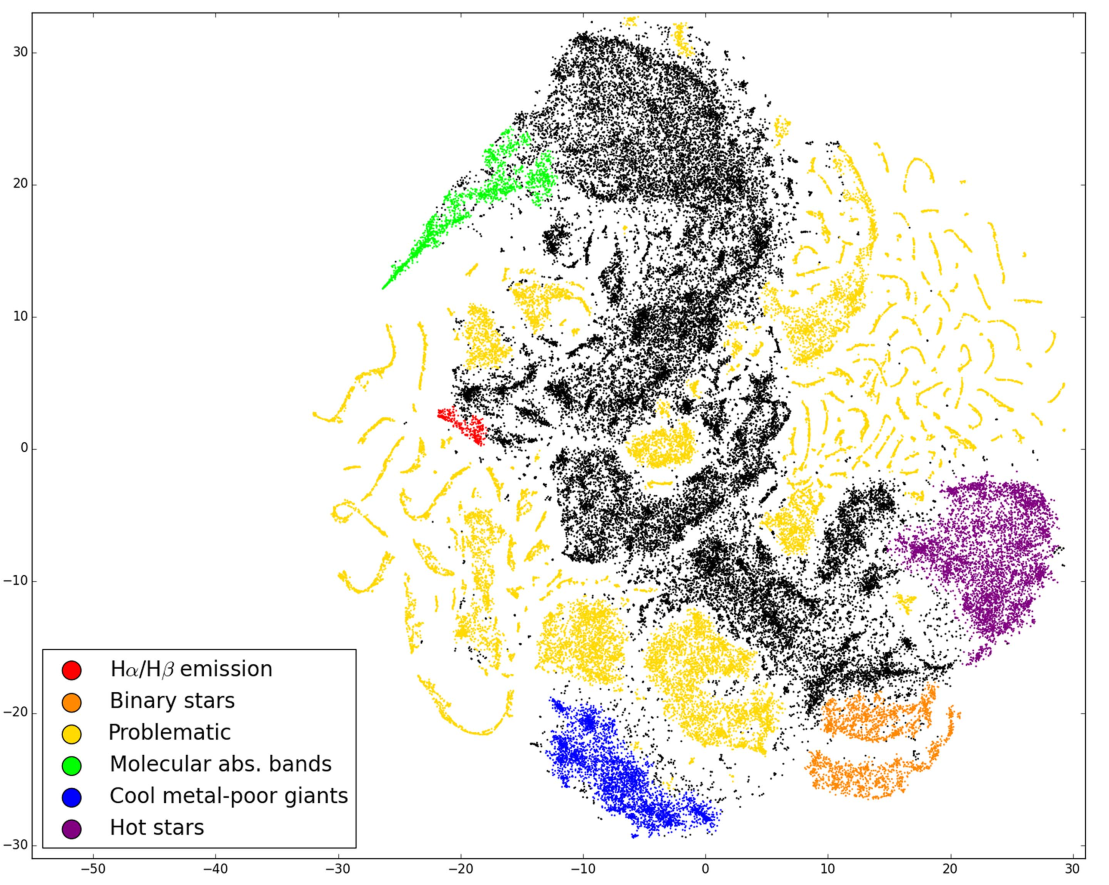
\includegraphics[scale=0.40]{figures/tsne traven.png}
\caption{The t-SNE plot with classified regions reproduced from Traven et al.\cite{traven2017galah}. The x and y axes do not have a physical meaning but serve as spanning vectors for the 2-dimensional space.}
\end{figure}

Using this method, Traven et al. classified six distinct stellar types and identified H$\upalpha$ and H$\upbeta$ emission-line spectra in GALAH DR1. These spectra were further examined and 18 P Cygni spectra were identified. The identification of P Cygni spectra was a sub-component of a broader study of stellar types in GALAH DR1. The authors note that the number identified was lower than expected which hints that there is significant scope to develop methods capabale of detecting a larger number of emission-line stars in the GALAH survey. Crucially, this method was not able to separate P Cygni spectra from double peaked spectra, emission superimposed on absorption and other emission-line spectra. When examining the t-SNE plot above, it is clear that the authors were not able to distinctly separate the H$\upalpha$ emission-line stars as a distinct cluster from the unclassified region (black) but rather fell back on manual tagging of this region on the projection space. This thesis will revisit this study in subsequent chapters and demonstrate a data driven method of separating P Cygni spectra from the aforementioned categories that can overcome some of the limitations mentioned above.

\subsection{Neural Networks as Anomaly Detectors: Using an Autoencoder on Data from GALAH DR3}

An autoencoder (AE) is a type of artificial neural network (ANN) that takes input data and reduces it to a pre-selected number of "latent features" that inhabit a low-dimensional vector space known as the latent space. The latent space can capture important features that exist in the original $d$-dimensional vector space. By processing $n$ samples of $d$-dimensional vectors, the autoencoder can then learn the latent space representation of the higher dimensional features. This is known as encoding. In the next portion of the network, the network then attempts to recover the original data from the latent vector space. The process that reduces a $d$-dimensional vector and vector space to a vector space of size $p$<$d$ is a dimensionality reduction process similar to PCA or t-SNE. The portion of the network that takes a $p$-dimensional vector from the latent space and projects it back to a $d$-dimensional vector space is essentially the inverse process of the dimensionality reduction procedure. This is known as a decoder. Since the original data is generated from the latent space, autoencoders fall into a class of ANNs called generative models (generative ANNs). Note that the latent space for an autoencoder is discrete. ANNs that can generate continuous latent spaces in this manner are known as variational autoencoders (VAEs) and are beyond the scope of this work. 

Autoencoders are widely used in anomaly detection applications\cite{sakurada2014anomaly}. If the autoencoder model is trained on non-anomalous data ("normal" data), the model will learn the latent space representation of non-anomalous data. Subsequently, if an anomalous data point is passed through the model, the autoencoder will attempt to generate this data from the latent space representation it has learned. Since the learned model was trained on non-anomalous data, the autoencoder will generate an inaccurate representation of the anomalous data. This leads a prediction error which can be used as a flag to to detect time-series as well as non time-series anomalies in data.

The GALAH survey is a general all-sky survey that can be expected to generate a significantly higher proportion non-anomalous spectra. Since DR3 is not biased towards young, violent, hot stars or stellar nurseries, we expect a significantly higher proportion of spectra to show "typical" (non-anomalous) H$\upalpha$ line profiles and indicate absorption. In this regime, an H$\upalpha$ emission-line, and consequently, P Cygni and inverse P Cygni spectra are rare and anomalous. If an autoencoder is trained on "normal looking" spectra which do not show emission lines near H$\upalpha$, it can be sensitive to H$\upalpha$ emission-line spectra. 

\begin{figure}[!htb]
\centering
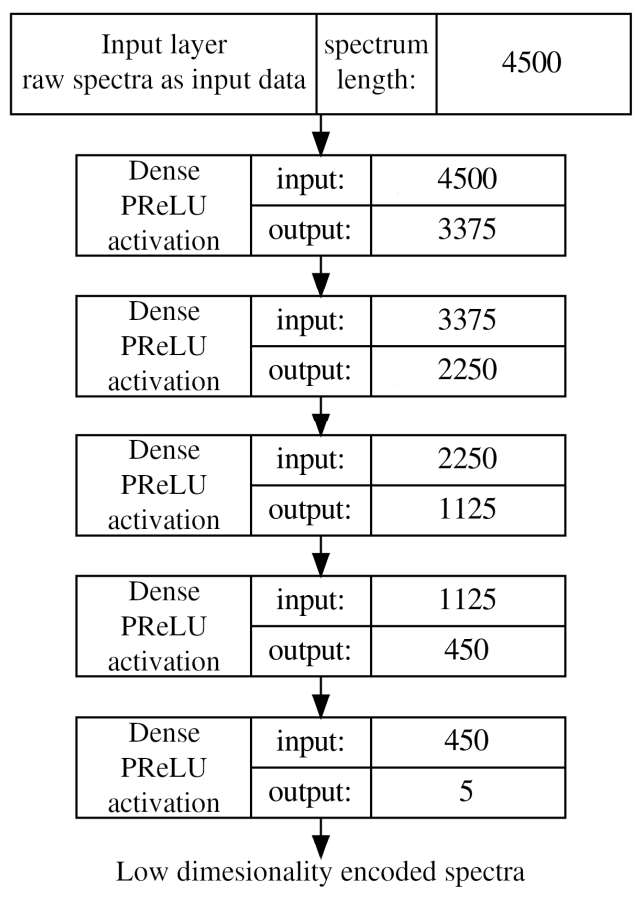
\includegraphics[scale=0.45]{figures/autoencoder.png}
\caption{An autoencoder architecture capable of detecting H$\upalpha$ emission-line spectra from DR3. Reproduced from Čotar et al.\cite{vcotar2021galah}}
\label{fig2.7}
\end{figure}

This method was used by Čotar et al. to detect H$\upalpha$ emission-line spectra in DR3 and other surveys\cite{vcotar2021galah}. The authors chose a network architecture that reduces a $d$-dimensional DR3 spectrum to a $p$-dimensional latent space representation. Here, $d$ = 4500 while $p$ = 5. Presumably, $p$ was set to 5 to potentially capture the primary stellar parameters and represent them within the latent space. The intervening layers and the final architecture that is capable of detecting H$\upalpha$ emission-line spectra is presented in Figure \ref{fig2.7} The authors did not further classify and detect P Cygni, inverse P Cygni and emission-line spectra using this method. 

\section{Concluding Remarks}

Regarding P Cygni stars and inverse P Cygni stars specifically, the literature is sparse and the available samples are few. For example a catalogueue of these spectra and stars do not exist at present. As recent as 2021, manual methods are being used to identify and classify P Cygni and inverse P Cygni spectra \cite{zhao2012lamost}. This limits the use of supervised machine learning methods and more importantly, can limit the science work that has been conducted on these spectra in the literature. Thus improvements to methods and the introduction of novel methods can lead to more emission-line spectra being identified and classified which in turn can lead to new science work on these stars. 

The use of machine learning has been a relatively new development in the field. As far as this author is aware, the use of t-SNE in 2017 is the first instance of using machine learning to identify and classify H$\upalpha$ emission-line spectra. However as this work will demonstrate in Chapter 5, it can be challenging to use t-SNE to classify P Cygni and inverse P Cygni spectra. 

Taking an anomaly detection or outlier detection approach such as Čotar et al. in 2021, and using a neural network architecture such as an autoencoder can be beneficial in reducing the search space of surveys such as GALAH from the total spectra available to only the potential emission-line spectra. However this method cannot be used to classify particular types and sub-species of emission-line stars such as P Cygni and inverse P Cygni. Similar to dimensionality reduction, this method can reduce the complexity of the problem by allowing the researcher to focus on only the most relevant data points when attempting to identify and classify emission-line spectra. Combined with other methods, this method can serve as a pre-processing step when identifying and classifying emission-line spectra. This work explores this idea fully in Chapters 4 and 6. 

Finally, popular unsupervised machine learning methods such as k-means as well as supervised machine learning methods such as logistic regression may not be suitable. The latter requires labeled training data\cite{zhang2021catalog} which this work did not posses. There exists evidence in literature that the former performed poorly on the task of identifying and classifying emission-line stars in a large scale spectroscopic survey in 2018\cite{garcia2018machine}. Due to time constraints, this work did not evaluate and consider these methods further.

